% Created by tikzDevice version 0.9 on 2015-12-31 00:08:52
% !TEX encoding = UTF-8 Unicode
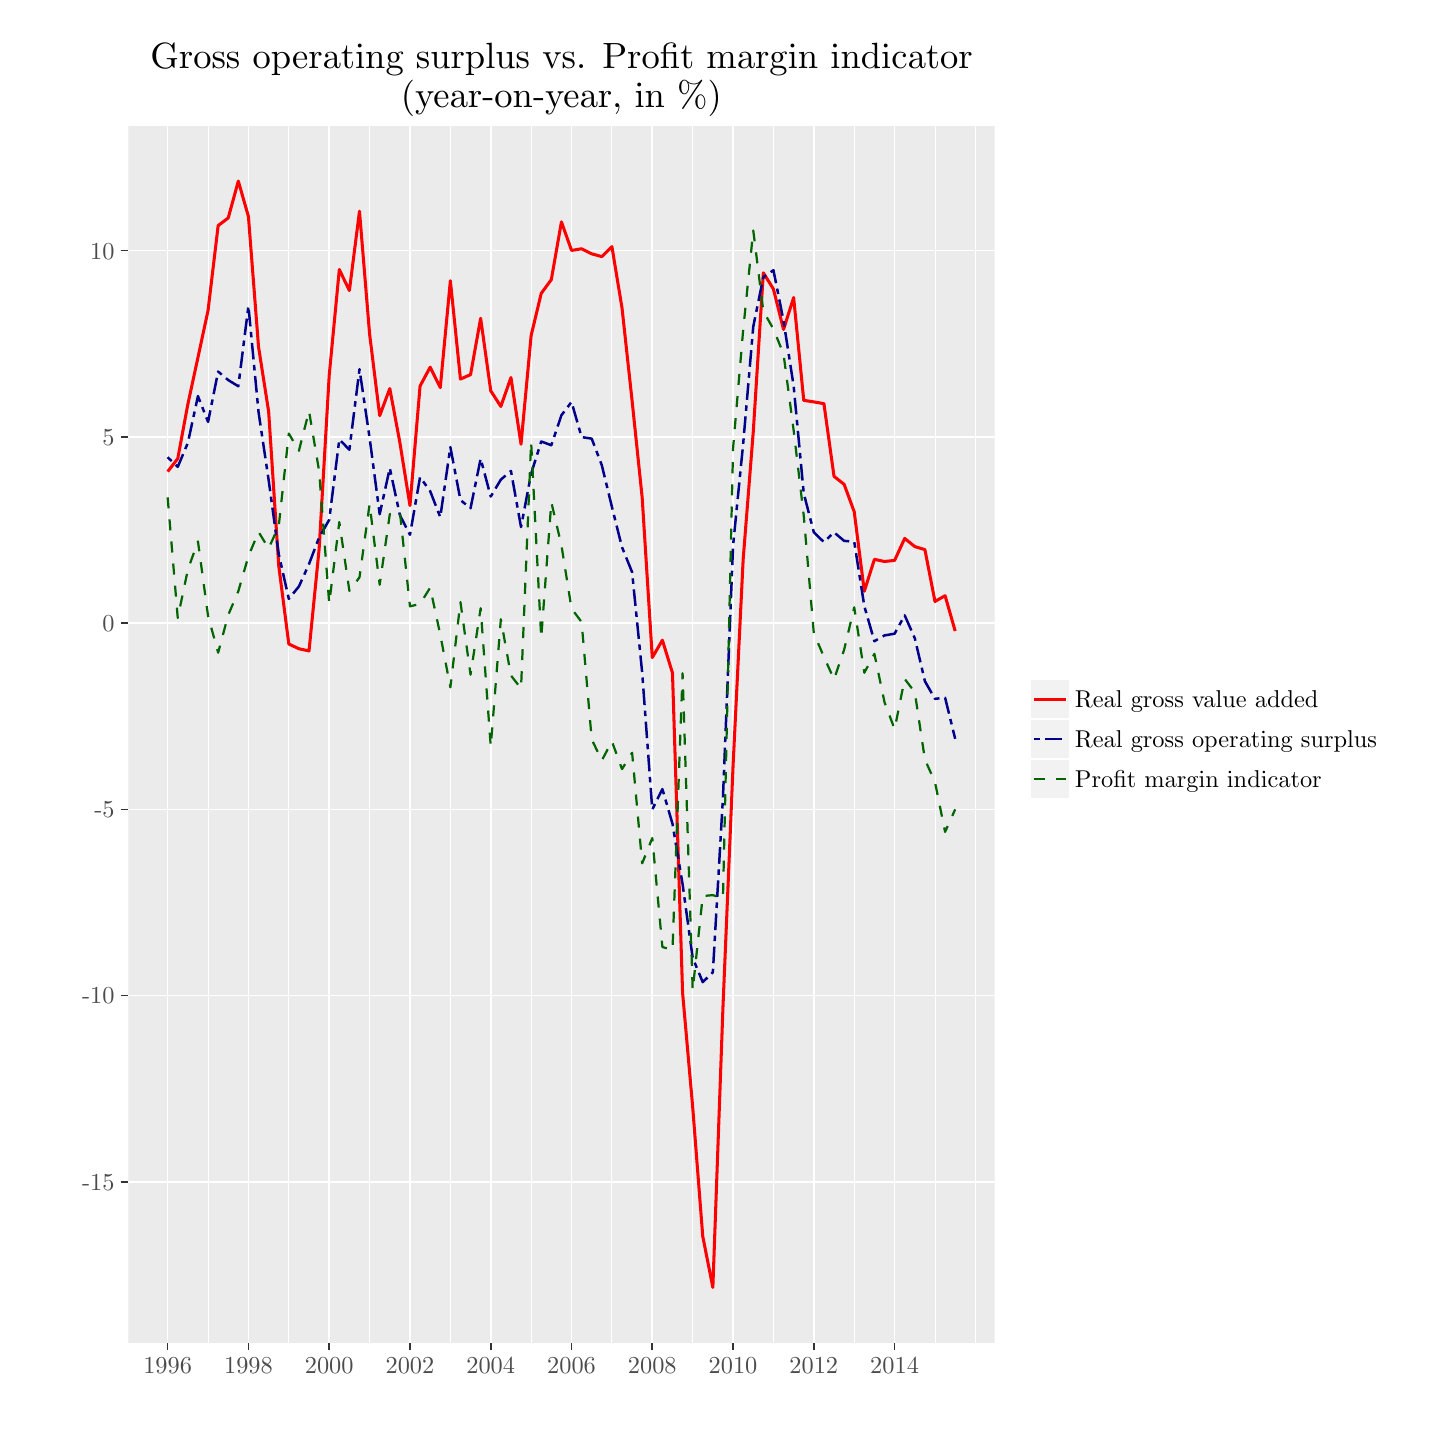
\begin{tikzpicture}[x=1pt,y=1pt]
\definecolor{fillColor}{RGB}{255,255,255}
\path[use as bounding box,fill=fillColor,fill opacity=0.00] (0,0) rectangle (505.89,505.89);
\begin{scope}
\path[clip] (  0.00,  0.00) rectangle (505.89,505.89);
\definecolor{drawColor}{RGB}{255,255,255}
\definecolor{fillColor}{RGB}{255,255,255}

\path[draw=drawColor,line width= 0.6pt,line join=round,line cap=round,fill=fillColor] (  0.00,  0.00) rectangle (505.89,505.89);
\end{scope}
\begin{scope}
\path[clip] ( 36.36, 30.69) rectangle (349.38,470.44);
\definecolor{fillColor}{gray}{0.92}

\path[fill=fillColor] ( 36.36, 30.69) rectangle (349.38,470.44);
\definecolor{drawColor}{RGB}{255,255,255}

\path[draw=drawColor,line width= 0.3pt,line join=round] ( 65.18, 30.69) --
	( 65.18,470.44);

\path[draw=drawColor,line width= 0.3pt,line join=round] ( 94.36, 30.69) --
	( 94.36,470.44);

\path[draw=drawColor,line width= 0.3pt,line join=round] (123.55, 30.69) --
	(123.55,470.44);

\path[draw=drawColor,line width= 0.3pt,line join=round] (152.74, 30.69) --
	(152.74,470.44);

\path[draw=drawColor,line width= 0.3pt,line join=round] (181.92, 30.69) --
	(181.92,470.44);

\path[draw=drawColor,line width= 0.3pt,line join=round] (211.11, 30.69) --
	(211.11,470.44);

\path[draw=drawColor,line width= 0.3pt,line join=round] (240.30, 30.69) --
	(240.30,470.44);

\path[draw=drawColor,line width= 0.3pt,line join=round] (269.48, 30.69) --
	(269.48,470.44);

\path[draw=drawColor,line width= 0.3pt,line join=round] (298.67, 30.69) --
	(298.67,470.44);

\path[draw=drawColor,line width= 0.3pt,line join=round] (327.85, 30.69) --
	(327.85,470.44);

\path[draw=drawColor,line width= 0.3pt,line join=round] (342.45, 30.69) --
	(342.45,470.44);

\path[draw=drawColor,line width= 0.6pt,line join=round] ( 36.36, 88.83) --
	(349.38, 88.83);

\path[draw=drawColor,line width= 0.6pt,line join=round] ( 36.36,156.13) --
	(349.38,156.13);

\path[draw=drawColor,line width= 0.6pt,line join=round] ( 36.36,223.42) --
	(349.38,223.42);

\path[draw=drawColor,line width= 0.6pt,line join=round] ( 36.36,290.72) --
	(349.38,290.72);

\path[draw=drawColor,line width= 0.6pt,line join=round] ( 36.36,358.01) --
	(349.38,358.01);

\path[draw=drawColor,line width= 0.6pt,line join=round] ( 36.36,425.31) --
	(349.38,425.31);

\path[draw=drawColor,line width= 0.6pt,line join=round] ( 50.58, 30.69) --
	( 50.58,470.44);

\path[draw=drawColor,line width= 0.6pt,line join=round] ( 79.77, 30.69) --
	( 79.77,470.44);

\path[draw=drawColor,line width= 0.6pt,line join=round] (108.96, 30.69) --
	(108.96,470.44);

\path[draw=drawColor,line width= 0.6pt,line join=round] (138.14, 30.69) --
	(138.14,470.44);

\path[draw=drawColor,line width= 0.6pt,line join=round] (167.33, 30.69) --
	(167.33,470.44);

\path[draw=drawColor,line width= 0.6pt,line join=round] (196.52, 30.69) --
	(196.52,470.44);

\path[draw=drawColor,line width= 0.6pt,line join=round] (225.70, 30.69) --
	(225.70,470.44);

\path[draw=drawColor,line width= 0.6pt,line join=round] (254.89, 30.69) --
	(254.89,470.44);

\path[draw=drawColor,line width= 0.6pt,line join=round] (284.07, 30.69) --
	(284.07,470.44);

\path[draw=drawColor,line width= 0.6pt,line join=round] (313.26, 30.69) --
	(313.26,470.44);
\definecolor{drawColor}{RGB}{255,0,0}

\path[draw=drawColor,line width= 1.1pt,line join=round] ( 50.58,345.48) --
	( 54.23,350.15) --
	( 57.88,369.83) --
	( 61.53,386.71) --
	( 65.18,403.73) --
	( 68.83,434.37) --
	( 72.47,437.12) --
	( 76.12,450.45) --
	( 79.77,437.63) --
	( 83.42,390.55) --
	( 87.07,367.19) --
	( 90.72,311.44) --
	( 94.36,283.17) --
	( 98.01,281.46) --
	(101.66,280.67) --
	(105.31,317.42) --
	(108.96,380.29) --
	(112.61,418.50) --
	(116.25,410.87) --
	(119.90,439.56) --
	(123.55,395.21) --
	(127.20,365.68) --
	(130.85,375.48) --
	(134.50,355.94) --
	(138.14,333.21) --
	(141.79,376.40) --
	(145.44,383.21) --
	(149.09,375.84) --
	(152.74,414.46) --
	(156.38,378.91) --
	(160.03,380.51) --
	(163.68,400.87) --
	(167.33,374.67) --
	(170.98,369.02) --
	(174.63,379.47) --
	(178.27,355.37) --
	(181.92,394.63) --
	(185.57,409.87) --
	(189.22,414.85) --
	(192.87,435.71) --
	(196.52,425.40) --
	(200.16,425.99) --
	(203.81,424.17) --
	(207.46,423.15) --
	(211.11,426.77) --
	(214.76,404.62) --
	(218.41,371.04) --
	(222.05,336.04) --
	(225.70,278.28) --
	(229.35,284.55) --
	(233.00,272.72) --
	(236.65,157.15) --
	(240.30,115.84) --
	(243.94, 69.11) --
	(247.59, 50.68) --
	(251.24,151.97) --
	(254.89,239.22) --
	(258.54,313.76) --
	(262.19,359.87) --
	(265.83,417.31) --
	(269.48,411.43) --
	(273.13,396.83) --
	(276.78,408.37) --
	(280.43,371.22) --
	(284.07,370.66) --
	(287.72,370.03) --
	(291.37,343.76) --
	(295.02,340.87) --
	(298.67,330.96) --
	(302.32,302.24) --
	(305.96,313.76) --
	(309.61,312.99) --
	(313.26,313.38) --
	(316.91,321.33) --
	(320.56,318.38) --
	(324.21,317.28) --
	(327.85,298.55) --
	(331.50,300.64) --
	(335.15,287.87);
\definecolor{drawColor}{RGB}{0,0,139}

\path[draw=drawColor,line width= 0.9pt,dash pattern=on 2pt off 2pt on 6pt off 2pt ,line join=round] ( 50.58,350.65) --
	( 54.23,347.19) --
	( 57.88,355.84) --
	( 61.53,372.76) --
	( 65.18,363.43) --
	( 68.83,381.62) --
	( 72.47,378.55) --
	( 76.12,376.31) --
	( 79.77,405.33) --
	( 83.42,367.00) --
	( 87.07,342.45) --
	( 90.72,315.64) --
	( 94.36,299.49) --
	( 98.01,303.96) --
	(101.66,312.07) --
	(105.31,321.70) --
	(108.96,328.05) --
	(112.61,357.11) --
	(116.25,353.37) --
	(119.90,382.47) --
	(123.55,357.67) --
	(127.20,330.08) --
	(130.85,346.73) --
	(134.50,329.72) --
	(138.14,322.64) --
	(141.79,343.47) --
	(145.44,338.41) --
	(149.09,329.01) --
	(152.74,354.34) --
	(156.38,335.18) --
	(160.03,332.24) --
	(163.68,350.14) --
	(167.33,336.46) --
	(170.98,342.58) --
	(174.63,345.70) --
	(178.27,325.44) --
	(181.92,344.70) --
	(185.57,356.36) --
	(189.22,354.99) --
	(192.87,365.84) --
	(196.52,370.64) --
	(200.16,357.94) --
	(203.81,357.38) --
	(207.46,347.78) --
	(211.11,332.74) --
	(214.76,318.17) --
	(218.41,309.13) --
	(222.05,272.81) --
	(225.70,223.38) --
	(229.35,230.75) --
	(233.00,218.23) --
	(236.65,196.39) --
	(240.30,169.75) --
	(243.94,160.98) --
	(247.59,164.57) --
	(251.24,227.67) --
	(254.89,318.73) --
	(258.54,355.52) --
	(262.19,397.86) --
	(265.83,415.74) --
	(269.48,418.25) --
	(273.13,399.94) --
	(276.78,376.43) --
	(280.43,337.65) --
	(284.07,323.54) --
	(287.72,320.00) --
	(291.37,323.53) --
	(295.02,320.44) --
	(298.67,320.14) --
	(302.32,296.85) --
	(305.96,284.19) --
	(309.61,286.27) --
	(313.26,286.91) --
	(316.91,293.53) --
	(320.56,285.25) --
	(324.21,269.73) --
	(327.85,263.35) --
	(331.50,263.80) --
	(335.15,248.93);
\definecolor{drawColor}{RGB}{0,100,0}

\path[draw=drawColor,line width= 0.8pt,dash pattern=on 4pt off 4pt ,line join=round] ( 50.58,336.17) --
	( 54.23,292.59) --
	( 57.88,310.04) --
	( 61.53,320.25) --
	( 65.18,293.30) --
	( 68.83,280.03) --
	( 72.47,293.67) --
	( 76.12,302.26) --
	( 79.77,314.91) --
	( 83.42,323.67) --
	( 87.07,317.73) --
	( 90.72,325.80) --
	( 94.36,359.22) --
	( 98.01,352.99) --
	(101.66,367.36) --
	(105.31,345.71) --
	(108.96,297.82) --
	(112.61,327.23) --
	(116.25,302.38) --
	(119.90,307.26) --
	(123.55,333.70) --
	(127.20,304.57) --
	(130.85,330.09) --
	(134.50,330.89) --
	(138.14,296.78) --
	(141.79,297.66) --
	(145.44,303.53) --
	(149.09,286.54) --
	(152.74,267.50) --
	(156.38,298.34) --
	(160.03,272.09) --
	(163.68,296.10) --
	(167.33,246.12) --
	(170.98,292.11) --
	(174.63,271.79) --
	(178.27,267.10) --
	(181.92,356.24) --
	(185.57,285.32) --
	(189.22,334.41) --
	(192.87,318.84) --
	(196.52,295.98) --
	(200.16,291.11) --
	(203.81,248.72) --
	(207.46,241.11) --
	(211.11,247.99) --
	(214.76,237.97) --
	(218.41,243.89) --
	(222.05,203.93) --
	(225.70,213.05) --
	(229.35,173.69) --
	(233.00,172.61) --
	(236.65,272.60) --
	(240.30,158.10) --
	(243.94,192.12) --
	(247.59,192.42) --
	(251.24,191.32) --
	(254.89,353.86) --
	(258.54,396.64) --
	(262.19,432.58) --
	(265.83,403.43) --
	(269.48,396.98) --
	(273.13,387.95) --
	(276.78,360.39) --
	(280.43,329.59) --
	(284.07,287.04) --
	(287.72,278.55) --
	(291.37,270.39) --
	(295.02,281.11) --
	(298.67,296.43) --
	(302.32,272.80) --
	(305.96,279.61) --
	(309.61,262.17) --
	(313.26,252.43) --
	(316.91,270.56) --
	(320.56,265.74) --
	(324.21,241.45) --
	(327.85,233.28) --
	(331.50,215.26) --
	(335.15,223.43);
\end{scope}
\begin{scope}
\path[clip] (  0.00,  0.00) rectangle (505.89,505.89);
\definecolor{drawColor}{gray}{0.30}

\node[text=drawColor,anchor=base east,inner sep=0pt, outer sep=0pt, scale=  0.88] at ( 31.41, 85.80) {-15};

\node[text=drawColor,anchor=base east,inner sep=0pt, outer sep=0pt, scale=  0.88] at ( 31.41,153.10) {-10};

\node[text=drawColor,anchor=base east,inner sep=0pt, outer sep=0pt, scale=  0.88] at ( 31.41,220.39) {-5};

\node[text=drawColor,anchor=base east,inner sep=0pt, outer sep=0pt, scale=  0.88] at ( 31.41,287.69) {0};

\node[text=drawColor,anchor=base east,inner sep=0pt, outer sep=0pt, scale=  0.88] at ( 31.41,354.98) {5};

\node[text=drawColor,anchor=base east,inner sep=0pt, outer sep=0pt, scale=  0.88] at ( 31.41,422.28) {10};
\end{scope}
\begin{scope}
\path[clip] (  0.00,  0.00) rectangle (505.89,505.89);
\definecolor{drawColor}{gray}{0.20}

\path[draw=drawColor,line width= 0.6pt,line join=round] ( 33.61, 88.83) --
	( 36.36, 88.83);

\path[draw=drawColor,line width= 0.6pt,line join=round] ( 33.61,156.13) --
	( 36.36,156.13);

\path[draw=drawColor,line width= 0.6pt,line join=round] ( 33.61,223.42) --
	( 36.36,223.42);

\path[draw=drawColor,line width= 0.6pt,line join=round] ( 33.61,290.72) --
	( 36.36,290.72);

\path[draw=drawColor,line width= 0.6pt,line join=round] ( 33.61,358.01) --
	( 36.36,358.01);

\path[draw=drawColor,line width= 0.6pt,line join=round] ( 33.61,425.31) --
	( 36.36,425.31);
\end{scope}
\begin{scope}
\path[clip] (  0.00,  0.00) rectangle (505.89,505.89);
\definecolor{drawColor}{gray}{0.20}

\path[draw=drawColor,line width= 0.6pt,line join=round] ( 50.58, 27.94) --
	( 50.58, 30.69);

\path[draw=drawColor,line width= 0.6pt,line join=round] ( 79.77, 27.94) --
	( 79.77, 30.69);

\path[draw=drawColor,line width= 0.6pt,line join=round] (108.96, 27.94) --
	(108.96, 30.69);

\path[draw=drawColor,line width= 0.6pt,line join=round] (138.14, 27.94) --
	(138.14, 30.69);

\path[draw=drawColor,line width= 0.6pt,line join=round] (167.33, 27.94) --
	(167.33, 30.69);

\path[draw=drawColor,line width= 0.6pt,line join=round] (196.52, 27.94) --
	(196.52, 30.69);

\path[draw=drawColor,line width= 0.6pt,line join=round] (225.70, 27.94) --
	(225.70, 30.69);

\path[draw=drawColor,line width= 0.6pt,line join=round] (254.89, 27.94) --
	(254.89, 30.69);

\path[draw=drawColor,line width= 0.6pt,line join=round] (284.07, 27.94) --
	(284.07, 30.69);

\path[draw=drawColor,line width= 0.6pt,line join=round] (313.26, 27.94) --
	(313.26, 30.69);
\end{scope}
\begin{scope}
\path[clip] (  0.00,  0.00) rectangle (505.89,505.89);
\definecolor{drawColor}{gray}{0.30}

\node[text=drawColor,anchor=base,inner sep=0pt, outer sep=0pt, scale=  0.88] at ( 50.58, 19.68) {1996};

\node[text=drawColor,anchor=base,inner sep=0pt, outer sep=0pt, scale=  0.88] at ( 79.77, 19.68) {1998};

\node[text=drawColor,anchor=base,inner sep=0pt, outer sep=0pt, scale=  0.88] at (108.96, 19.68) {2000};

\node[text=drawColor,anchor=base,inner sep=0pt, outer sep=0pt, scale=  0.88] at (138.14, 19.68) {2002};

\node[text=drawColor,anchor=base,inner sep=0pt, outer sep=0pt, scale=  0.88] at (167.33, 19.68) {2004};

\node[text=drawColor,anchor=base,inner sep=0pt, outer sep=0pt, scale=  0.88] at (196.52, 19.68) {2006};

\node[text=drawColor,anchor=base,inner sep=0pt, outer sep=0pt, scale=  0.88] at (225.70, 19.68) {2008};

\node[text=drawColor,anchor=base,inner sep=0pt, outer sep=0pt, scale=  0.88] at (254.89, 19.68) {2010};

\node[text=drawColor,anchor=base,inner sep=0pt, outer sep=0pt, scale=  0.88] at (284.07, 19.68) {2012};

\node[text=drawColor,anchor=base,inner sep=0pt, outer sep=0pt, scale=  0.88] at (313.26, 19.68) {2014};
\end{scope}
\begin{scope}
\path[clip] (  0.00,  0.00) rectangle (505.89,505.89);
\definecolor{fillColor}{RGB}{255,255,255}

\path[fill=fillColor] (357.91,222.81) rectangle (491.85,278.32);
\end{scope}
\begin{scope}
\path[clip] (  0.00,  0.00) rectangle (505.89,505.89);
\definecolor{drawColor}{RGB}{255,255,255}
\definecolor{fillColor}{gray}{0.95}

\path[draw=drawColor,line width= 0.6pt,line join=round,line cap=round,fill=fillColor] (362.18,255.99) rectangle (376.64,270.44);
\end{scope}
\begin{scope}
\path[clip] (  0.00,  0.00) rectangle (505.89,505.89);
\definecolor{drawColor}{RGB}{255,0,0}

\path[draw=drawColor,line width= 1.1pt,line join=round] (363.63,263.21) -- (375.19,263.21);
\end{scope}
\begin{scope}
\path[clip] (  0.00,  0.00) rectangle (505.89,505.89);
\definecolor{drawColor}{RGB}{255,255,255}
\definecolor{fillColor}{gray}{0.95}

\path[draw=drawColor,line width= 0.6pt,line join=round,line cap=round,fill=fillColor] (362.18,241.53) rectangle (376.64,255.99);
\end{scope}
\begin{scope}
\path[clip] (  0.00,  0.00) rectangle (505.89,505.89);
\definecolor{drawColor}{RGB}{0,0,139}

\path[draw=drawColor,line width= 0.9pt,dash pattern=on 2pt off 2pt on 6pt off 2pt ,line join=round] (363.63,248.76) -- (375.19,248.76);
\end{scope}
\begin{scope}
\path[clip] (  0.00,  0.00) rectangle (505.89,505.89);
\definecolor{drawColor}{RGB}{255,255,255}
\definecolor{fillColor}{gray}{0.95}

\path[draw=drawColor,line width= 0.6pt,line join=round,line cap=round,fill=fillColor] (362.18,227.08) rectangle (376.64,241.53);
\end{scope}
\begin{scope}
\path[clip] (  0.00,  0.00) rectangle (505.89,505.89);
\definecolor{drawColor}{RGB}{0,100,0}

\path[draw=drawColor,line width= 0.8pt,dash pattern=on 4pt off 4pt ,line join=round] (363.63,234.30) -- (375.19,234.30);
\end{scope}
\begin{scope}
\path[clip] (  0.00,  0.00) rectangle (505.89,505.89);
\definecolor{drawColor}{RGB}{0,0,0}

\node[text=drawColor,anchor=base west,inner sep=0pt, outer sep=0pt, scale=  0.88] at (378.44,260.18) {Real gross value added};
\end{scope}
\begin{scope}
\path[clip] (  0.00,  0.00) rectangle (505.89,505.89);
\definecolor{drawColor}{RGB}{0,0,0}

\node[text=drawColor,anchor=base west,inner sep=0pt, outer sep=0pt, scale=  0.88] at (378.44,245.73) {Real gross operating surplus};
\end{scope}
\begin{scope}
\path[clip] (  0.00,  0.00) rectangle (505.89,505.89);
\definecolor{drawColor}{RGB}{0,0,0}

\node[text=drawColor,anchor=base west,inner sep=0pt, outer sep=0pt, scale=  0.88] at (378.44,231.27) {Profit margin indicator};
\end{scope}
\begin{scope}
\path[clip] (  0.00,  0.00) rectangle (505.89,505.89);
\definecolor{drawColor}{RGB}{0,0,0}

\node[text=drawColor,anchor=base,inner sep=0pt, outer sep=0pt, scale=  1.32] at (192.87,491.30) {Gross operating surplus vs. Profit margin indicator };

\node[text=drawColor,anchor=base,inner sep=0pt, outer sep=0pt, scale=  1.32] at (192.87,477.04) { (year-on-year, in {\%})};
\end{scope}
\end{tikzpicture}
